\documentclass[11pt,titlepage,a4paper]{report}

%INCLUSIONE PACCHETTI
%---------------------------------------------
\usepackage[italian]{babel}
\usepackage{fancyhdr}
\usepackage{graphicx}
\graphicspath{{./pics/}} % cartella di salvataggio immagini

% STILE DI PAGINA
%---------------------------------------------
\pagestyle{fancy}
\renewcommand{\sectionmark}[1]{\markright{\thesection.\ #1}}
\lhead{\nouppercase{\rightmark}}
\rhead{\nouppercase{\leftmark}}
\renewcommand{\chaptermark}[1]{%
\markboth{\thechapter.\ #1}{}}

%Ridefinisco lo stile plain della pagina
\fancypagestyle{plain}{%
	\lhead{
\includegraphics[height=50pt]{logo.eps}}
	\chead{}
	\rhead{HappyCode inc \\ happycodeinc@gmail.com}
	\lfoot{BR-jsys}
	\cfoot{\thepage}
	\renewcommand{\headrulewidth}{1pt}
	\renewcommand{\footrulewidth}{1pt}
}

\begin{document}


%definizione variabili 
\newcommand{\lv}{1.3 } % latest version
\newcommand{\Glossario}{ Glossario.1.4.pdf }
%fine definizione variabili

\hyphenation{glos-sa-rio es-pli-ci-to ve-ri-fi-ca-re re-po-si-to-ry se-gna-la-ta coe-ren-za}
\begin{titlepage}
\begin{center}
\vspace*{0.5in}

\includegraphics{logo.eps}
\vspace*{0.2in}

{\Large \textbf{BR-jsys}}
{\Large \emph{business rules} per sistemi gestionali in architettura J2EE } 
\vspace{2in}

\LARGE \textbf {PIANO DI PROGETTO}
\par\rule{10cm}{0.4pt} \par {\large Versione \lv - \today}


\end{center}
\end{titlepage}
\vspace*{0.5in}


\begin{center}
\thispagestyle{plain}
\begin{table}[htbp]
\large{
\begin{tabular}{l}
\Large{\textbf{\textsf{Capitolato: ''BR-jsys``}}} \\
\begin{tabular}{||p{6cm}||p{6cm}||} \hline
\textbf{Data creazione:} & 2007/11/21 \\ \hline
\textbf{Versione:} & \lv \\ \hline
% ----------------------------------------------------------------------------autori
\textbf{Stato del documento:} & formale, esterno \\ \hline
\textbf{Revisione RR} &           \\ \hline
\textbf{Redazione:} & Elena Trivellato \\ \hline
\textbf{Revisione:} & Marco Tessarotto \\ \hline
\textbf{Approvazione:} Elena Trivellato & \\ \hline
\textbf{Revisione RPD}     \\ \hline
\textbf{Redazione:} & Mattia Meroi \\ \hline
\textbf{Revisione:} & Elena Trivellato, Filippo Carraro \\ \hline
\textbf{Approvazione:}  & Mattia Meroi \\ \hline
\end{tabular} \\
\end{tabular}
}
\end{table}

\begin{table}[hbtp]
\large{
\begin{tabular}{l}
\Large{\textbf{\textsf{Lista di distribuzione}}} \\
\begin{tabular}{||p{6cm}||p{6cm}||} \hline
%  -------------------------------------------------------------lista di distribuzione
{HappyCode inc}& Gruppo di lavoro\\ \hline
{Tullio Vardanega, Renato Conte}& Rappresentanti del committente \\ \hline 
{Zucchetti S.r.l}& Azienda committente\\ \hline
\end{tabular} \\
\end{tabular}
}
\end{table}
\begin{table}[hbtp]
\large{
\begin{tabular}{l}
\Large{\textbf{\textsf{Diario delle modifiche}}} \\
\begin{tabular}{||p{2cm}||p{3.5cm}||p{6cm}||}
\hline
\textbf{Versione} & \textbf{Data rilascio} & \textbf{Descrizione} \\ \hline
1.3 & 25/01/2008 & Aggiunta tabelle delle ore effettivamente impiegate in fase di analisi \\ \hline
1.2 & 23/01/2008 & Aggiunto carico totale delle risorse preventivo \\ \hline
1.1 & 22/01/2008 & Modifica al layout dei documenti.\\ \hline
1.0 & 21/12/2007 & Documento sottoposto a revisionamento automatico.\\ \hline
0.5 & 05/12/2007 & Aggiunto riferimento diagramma di Gantt \\ \hline
0.4 & 29/11/2007 & Stesura completa del documento. \\ \hline
0.3 & 25/11/2007 & Assegnazione dei ruoli ai componenti del gruppo. \\ \hline
0.2 & 23/11/2007 & Riviste al ribasso le ore di programmazione. \\ \hline
0.1 & 21/11/2007 & Stesura preliminare del documento. \\ \hline

\end{tabular} \\
\end{tabular}

}
\end{table}
\end{center}


\tableofcontents 


\chapter{Introduzione}
\section{Scopo del documento}
Questo documento rappresenta il piano di progetto preliminare
del capitolato d'appalto per il sistema "Business Rules per sistemi
gestionali in architettura J2EE BR-jsys". 
Qui \`e riportata la divisione dei ruoli e il costo complessivo del
sistema in base ai ruoli e alle ore impegnate.

\section{Glossario}
Il glossario viene fornito come file esterno chiamato \Glossario .

\chapter{Ruoli}
\section{Definizione ruoli}
Riportiamo la tabella 1 nella quale vediamo l'impegno
complessivo in base ai ruoli di progetto nelle quattro
macrofasi previste dal ciclo di vita del nostro software.


\begin{table}[hbtp]
\large{
\begin{tabular}{l}
\Large{\textbf{\textsf{Tabella dei Ruoli}}} \\
\begin{tabular}{||p{3cm}||p{2cm}||p{2cm}||p{2cm}||p{2cm}||}
\hline
\textbf{Ruoli} & \textbf{Analisi} & \textbf{Progett.} & \textbf{Sviluppo}
& \textbf{Verifica}\\ \hline
{Responsabile}&10&10&10&9 \\ \hline 
{Amministratore} &10&10&10&10\\ \hline
{Analista}& 58&20&5&0 \\ \hline
{Progettista}&29&75&25&0 \\ \hline
{Programmatore}&0&5&60&55 \\ \hline
{Verificatore}& 30&30&90&95 \\ \hline
{Totale}& 137&150&200&169 \\ \hline
\end{tabular} \\ 
\end{tabular}
}

\end{table}

Mostriamo con un grafico in che misura incide ciascun ruolo per ogni macrofase,
cio\`e vediamo graficamente come ogni ruolo di progetto contribuisce a formare 
il totale delle ore di ciascuna delle quattro fasi di lavoro:
\begin{center}
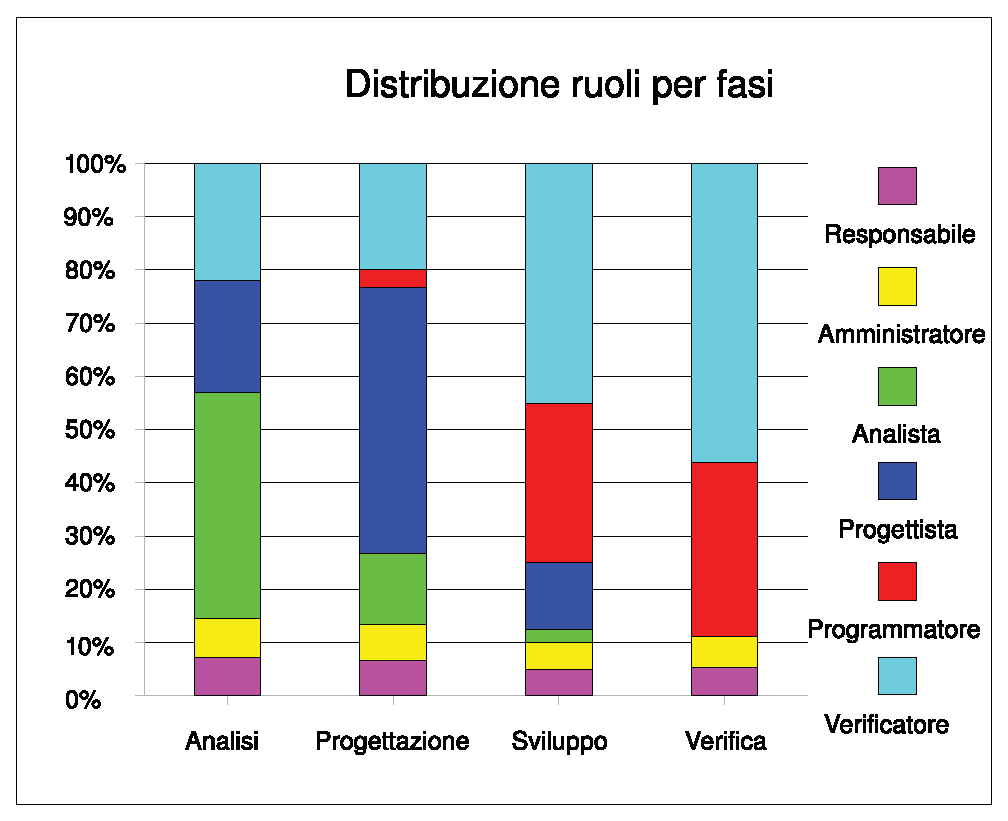
\includegraphics [width=1\textwidth] {ruoliperFasi.eps}
\end{center}

\section{Incidenza percentuale}
Riportiamo in questa tabella il peso percentuale di ciascun ruolo nelle ore
complessive previste di realizzazione del prodotto:
\begin{table}[hbtp]
\large{
\begin{tabular}{l}
\Large{\textbf{\textsf{Tabella delle percentuali dei ruoli}}} \\
\begin{tabular}{||p{6cm}||p{4cm}||}
\hline
\textbf{Ruoli} & \textbf{Percentuali}\\ \hline
{Responsabile}&6\\ \hline 
{Amministratore} &6\\ \hline
{Analista} &13 \\ \hline
{Progettista} &17\\ \hline
{Programmatore} &19\\ \hline
{Verificatore} &39 \\ \hline
{Totale} &100 \\ \hline
\end{tabular} \\
\end{tabular}
}
\end{table}

Evidenziamo la distribuzione delle ore tra i vari ruoli con un grafico; 
a differenza di prima qui abbiamo una visione globale riguardante 
tutto il ciclo di vita del software:


\begin{center}
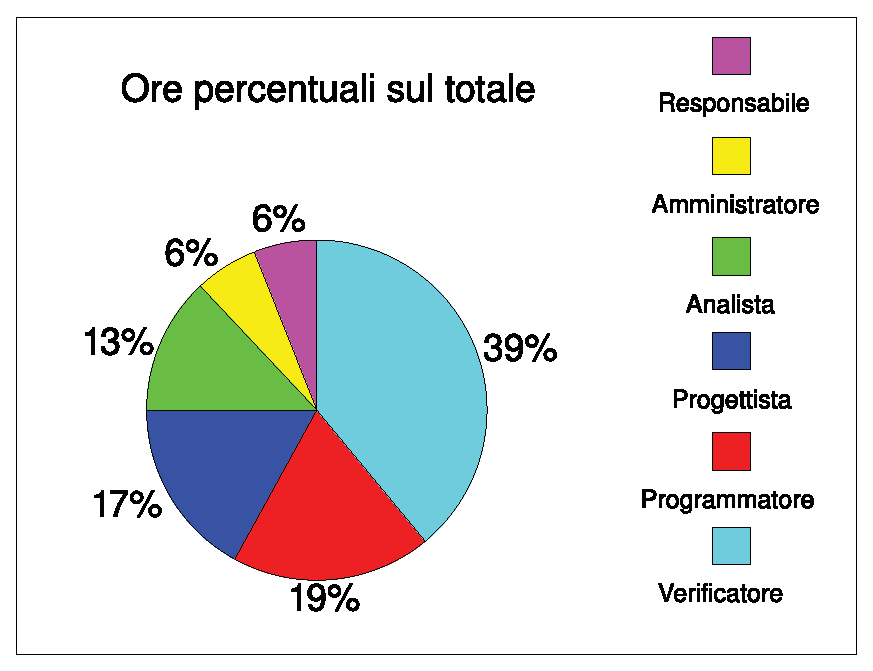
\includegraphics [width=1\textwidth] {orePercentuali.eps}
\end{center}


\section{Assegnazione dei ruoli e delle ore a ciascun membro}
In questa parte del documento mostriamo come i vari ruoli siano distribuiti 
tra i componenti del gruppo nelle quattro macrofasi
Nelle previsioni in questa fase di lavoro l'attivit\`a di progettazione 
doveva richiedere solo 5 ore del nostro tempo; in realt\`a sono state 
dedicate a questa attivit\`a ben 29 ore in questa fase. I tempi previsti
per le altre attivit\`a sono stati quasi tutti rispettati, ad eccezione del
l'analisi dei requisiti che ha richiesto 2 ore in meno del previsto.

\begin{table}[hbtp]
\large{
\begin{tabular}{l}
\Large{\textbf{\textsf{Fase di Analisi (Consuntivo al 26/01/08) - 1}}} \\
\begin{tabular}{||p{3.5cm}||p{2cm}||p{2cm}||p{2cm}||p{2cm}||}
\hline
\textbf{Membro} & \textbf{Respon.} & \textbf{Ammin.} & \textbf{Analista}
& \textbf{Progett.}\\ \hline
{Appon Luca}&0&5&8&3 \\ \hline 
{Bortolato Michele} &2&0&9&7\\ \hline
{Carraro Filippo}&0&5&8&4 \\ \hline
{Meroi Mattia}&6&0&6&3\\ \hline
{Tessarotto Marco} &0&0&9&7\\ \hline
{Trivellato Alessia} &0&0&9&3 \\ \hline
{Trivellato Elena} &2&0&9&2 \\ \hline
{Totale}& 10&10&58&29 \\ \hline
\end{tabular} \\
\end{tabular}
}
\end{table}

\begin{table}[hbtp]
\large{
\begin{tabular}{l}
\Large{\textbf{\textsf{Fase di analisi (Consuntivo al 26/01/08) - 2}}} \\
\begin{tabular}{||p{3.5cm}||p{2cm}||p{2cm}||p{2cm}||p{2cm}||}
\hline
\textbf{Membro} & \textbf{Program} & \textbf{Verif.} & \textbf{Totale}\\ \hline
{Appon Luca}&0&3&17 \\ \hline 
{Bortolato Michele} &0&3&16\\ \hline
{Carraro Filippo}&0&3&16 \\ \hline
{Meroi Mattia}&0&4&17\\ \hline
{Tessarotto Marco} &0&4&16\\ \hline
{Trivellato Alessia} &0&7&16 \\ \hline
{Trivellato Elena} &0&6&17 \\ \hline
{Totale} &0&30&115 \\ \hline
\end{tabular} \\
\end{tabular}
}
\end{table}


\begin{table}[hbtp]
\large{
\begin{tabular}{l}
\Large{\textbf{\textsf{Fase di Progettazione (Preventivo) - 1}}} \\
\begin{tabular}{||p{3.5cm}||p{2cm}||p{2cm}||p{2cm}||p{2cm}||}
\hline
\textbf{Membro} & \textbf{Respon.} & \textbf{Ammin.} & \textbf{Analista} & \textbf{Progett.}\\ \hline
{Appon Luca}&4&0&2&10 \\ \hline 
{Bortolato Michele} &4&0&2&10\\ \hline
{Carraro Filippo}&0&0&4&12 \\ \hline
{Meroi Mattia}&0&5&3&10\\ \hline
{Tessarotto Marco} &0&0&4&10\\ \hline
{Trivellato Alessia} &0&5&2&12 \\ \hline
{Trivellato Elena} &2&0&3&11 \\ \hline
{Totale}& 10&10&20&75 \\ \hline
\end{tabular} \\
\end{tabular}
}
\end{table}

\begin{table}[hbtp]
\large{
\begin{tabular}{l}
\Large{\textbf{\textsf{Fase di Progettazione (Preventivo) - 2}}} \\
\begin{tabular}{||p{3.5cm}||p{2cm}||p{2cm}||p{2cm}||p{2cm}||}
\hline
\textbf{Membro} & \textbf{Program} & \textbf{Verif.} & \textbf{Totale}\\ \hline
{Appon Luca}&0&5&21 \\ \hline 
{Bortolato Michele} &0&6&22\\ \hline
{Carraro Filippo}&0&5&21 \\ \hline
{Meroi Mattia}&0&3&21\\ \hline
{Tessarotto Marco} &5&3&22\\ \hline
{Trivellato Alessia} &0&3&22 \\ \hline
{Trivellato Elena} &0&5&21 \\ \hline
{Totale}& 5&30&150 \\ \hline
\end{tabular} \\
\end{tabular}
}
\end{table}


\begin{table}[hbtp]
\large{
\begin{tabular}{l}
\Large{\textbf{\textsf{Fase di Sviluppo (Preventivo) - 1}}} \\
\begin{tabular}{||p{3.5cm}||p{2cm}||p{2cm}||p{2cm}||p{2cm}||}
\hline
\textbf{Membro} & \textbf{Respon.} & \textbf{Ammin.} & \textbf{Analista} & \textbf{Progett.}\\ \hline
{Appon Luca}&0&0&2&5 \\ \hline 
{Bortolato Michele} &0&2&0&3\\ \hline
{Carraro Filippo}&5&0&0&4 \\ \hline
{Meroi Mattia}&0&0&3&4\\ \hline
{Tessarotto Marco} &5&6&0&3\\ \hline
{Trivellato Alessia} &0&2&0&3 \\ \hline
{Trivellato Elena} &0&0&0&3 \\ \hline
{Totale}& 10&10&5&25 \\ \hline
\end{tabular} \\
\end{tabular}
}
\end{table}

\begin{table}[hbtp]
\large{
\begin{tabular}{l}
\Large{\textbf{\textsf{Fase di Sviluppo (Preventivo) - 2}}} \\
\begin{tabular}{||p{3.5cm}||p{2cm}||p{2cm}||p{2cm}||p{2cm}||}
\hline
\textbf{Membro} & \textbf{Program} & \textbf{Verif.} & \textbf{Totale}\\ \hline
{Appon Luca}&10&12&29 \\ \hline 
{Bortolato Michele} &12&10&27\\ \hline
{Carraro Filippo}&8&12&29 \\ \hline
{Meroi Mattia}&12&9&28\\ \hline
{Tessarotto Marco} &4&11&29\\ \hline
{Trivellato Alessia} &7&17&29 \\ \hline
{Trivellato Elena} &7&19&29 \\ \hline
{Totale}& 60&90&200 \\ \hline
\end{tabular} \\
\end{tabular}
}
\end{table}


\begin{table}[hbtp]
\large{
\begin{tabular}{l}
\Large{\textbf{\textsf{Fase di Verifica (Preventivo) - 1}}} \\
\begin{tabular}{||p{3.5cm}||p{2cm}||p{2cm}||p{2cm}||p{2cm}||} \hline
\textbf{Membro} & \textbf{Respon.} & \textbf{Ammin.} & \textbf{Analista} & \textbf{Progett.}\\ \hline
{Appon Luca}&2&0&0&0 \\ \hline 
{Bortolato Michele} &0&5&0&0\\ \hline
{Carraro Filippo}&0&0&0&0 \\ \hline
{Meroi Mattia}&0&0&0&0\\ \hline
{Tessarotto Marco} &0&0&0&0\\ \hline
{Trivellato Alessia} &5&0&0&0 \\ \hline
{Trivellato Elena} &2&5&0&0 \\ \hline
{Totale}& 9&10&0&0 \\ \hline
\end{tabular} \\
\end{tabular}
}
\end{table}

\begin{table}[hbtp]
\large{
\begin{tabular}{l}
\Large{\textbf{\textsf{Fase di Verifica (Preventivo) - 2}}} \\
\begin{tabular}{||p{3.5cm}||p{2cm}||p{2cm}||p{2cm}||p{2cm}||} \hline
\textbf{Membro} & \textbf{Program} & \textbf{Verif.} & \textbf{Totale}\\ \hline
{Appon Luca}&6&16&24 \\ \hline
{Bortolato Michele} &3&17&25\\ \hline
{Carraro Filippo}&10&14&24 \\ \hline
{Meroi Mattia}&7&17&24\\ \hline
{Tessarotto Marco} &7&17&249\\ \hline
{Trivellato Alessia} &11&8&24 \\ \hline
{Trivellato Elena} &11&6&24 \\ \hline
{Totale} &55&95&169 \\ \hline
\end{tabular} \\
\end{tabular}
}
\end{table}

\newpage

\section{Carico totale di ore per ciascun componente}
In questa sezione vediamo in che misura (numero di ore) ogni componente collabora alla 
realizzazione del progetto in ogni macrofase e globalmente.
Essendo aumentate le ore di progettazione, anche il carico totale 
per ciascuna risorsa umana \`e leggermente aumentato.

\begin{table}[hbtp]
\large{
\begin{tabular}{l}
\Large{\textbf{\textsf{Carico totale delle risorse (Consuntivo al 26/01/08) - 1}}} \\
\begin{tabular}{||p{3.5cm}||p{2cm}||p{2cm}||p{2cm}||p{2cm}||} \hline
\textbf{Membro} & \textbf{Respon.} & \textbf{Ammin.} & \textbf{Analista} & \textbf{Progett.}\\ \hline
{Appon Luca}&6&5&12&18 \\ \hline
{Bortolato Michele} &6&7&11&20\\ \hline
{Carraro Filippo}&5&5&12&20 \\ \hline
{Meroi Mattia}&6&5&12&17\\ \hline
{Tessarotto Marco} &5&6&13&20\\ \hline
{Trivellato Alessia} &5&7&11&18 \\ \hline
{Trivellato Elena} &6&5&12&16 \\ \hline
{Totale}& 39&40&85&105 \\ \hline
\end{tabular} \\
\end{tabular}
}
\end{table}

\begin{table}[hbtp]
\large{
\begin{tabular}{l}
\Large{\textbf{\textsf{Carico totale delle risorse (Consuntivo al 26/01/08) - 2}}} \\
\begin{tabular}{||p{3.5cm}||p{2cm}||p{2cm}||p{2cm}||p{2cm}||} \hline
\textbf{Membro} & \textbf{Program} & \textbf{Verif.} & \textbf{Totale}\\ \hline
{Appon Luca}&16&36&91 \\ \hline 
{Bortolato Michele} &15&36&90\\ \hline
{Carraro Filippo}&18&34&90 \\ \hline
{Meroi Mattia}&19&33&90\\ \hline
{Tessarotto Marco} &16&35&91\\ \hline
{Trivellato Alessia} &18&35&91 \\ \hline
{Trivellato Elena} &18&36&91 \\ \hline
{Totale} &120&245&634 \\ \hline
\end{tabular} \\
\end{tabular}
}
\end{table}


\chapter{Costi}
\section{Costo orario per ogni ruolo}
Evidenziamo il costo orario di ciascun ruolo di progetto
\begin{table}[hbtp]
\large{
\begin{tabular}{l}
\Large{\textbf{\textsf{Tabella dei costi orari}}} \\
\begin{tabular}{||p{6cm}||p{5cm}||}\hline
\textbf{Ruoli} & \textbf{Costo orario in Euro}\\ \hline
{Responsabile}&30\\ \hline 
{Amministratore} &18\\ \hline
{Analista} &25 \\ \hline
{Progettista} &20 \\ \hline
{Programmatore} &15\\ \hline
{Verificatore} &15 \\ \hline
\end{tabular} \\
\end{tabular}
}
\end{table}

\section{Costo totale per ogni ruolo}
Evidenziamo il costo totale di ciascun ruolo di progetto e la sua incidenza
percentuale sul totale di spesa prevista.
%\begin{table}[hbtp]
%\large{
%\begin{tabular}{l}
%\Large{\textbf{\textsf{Tabella dei costi Totali (Preventivo)}}} \\
%\begin{tabular}{||p{4cm}||p{3cm}||p{3cm}||}
%\hline
%\textbf{Ruoli} & \textbf{Costo Totale}& \textbf{Costo Percentuale}\\
%\hline
%{Responsabile}&1.170&10\\ 
%\hline 
%{Amministratore} &720&6\\ 
%\hline
%{Analista} &2.125&18 \\
%\hline
%{Progettista} &2.100&18 \\
%\hline
%{Programmatore} &1.800&16\\
%\hline
%{Verificatore} &3.675&32 \\
%\hline
%{Totale} &11.590&100 \\
%\hline
%\end{tabular} \\
%\end{tabular}
%}
%\end{table}

Vediamo che l'incremento di ore effettive&2&0&3&11 rispetto a quelle previste ha causato
anche un aumento del costo complessivo del lavoro di 430.00 euro

\begin{table}[hbtp]
\large{
\begin{tabular}{l}
\Large{\textbf{\textsf{Tabella dei costi Totali (Consuntivo al 21/01/08)}}} \\
\begin{tabular}{||p{4cm}||p{3cm}||p{3cm}||} \hline
\textbf{Ruoli} & \textbf{Costo Totale}& \textbf{Costo Percentuale}\\ \hline
{Responsabile}&1.170&10\\ \hline 
{Amministratore} &720&6\\ \hline
{Analista} &2.075&18 \\ \hline
{Progettista} &2.580&18 \\ \hline
{Programmatore} &1.800&16\\ \hline
{Verificatore} &3.675&32 \\ \hline
{Totale} &12.020&100 \\ \hline
\end{tabular} \\
\end{tabular}
}
\end{table}


Evidenziamo come il costo di ciascun ruolo incide in percentuale
sul totale con un grafico:
\begin{center}
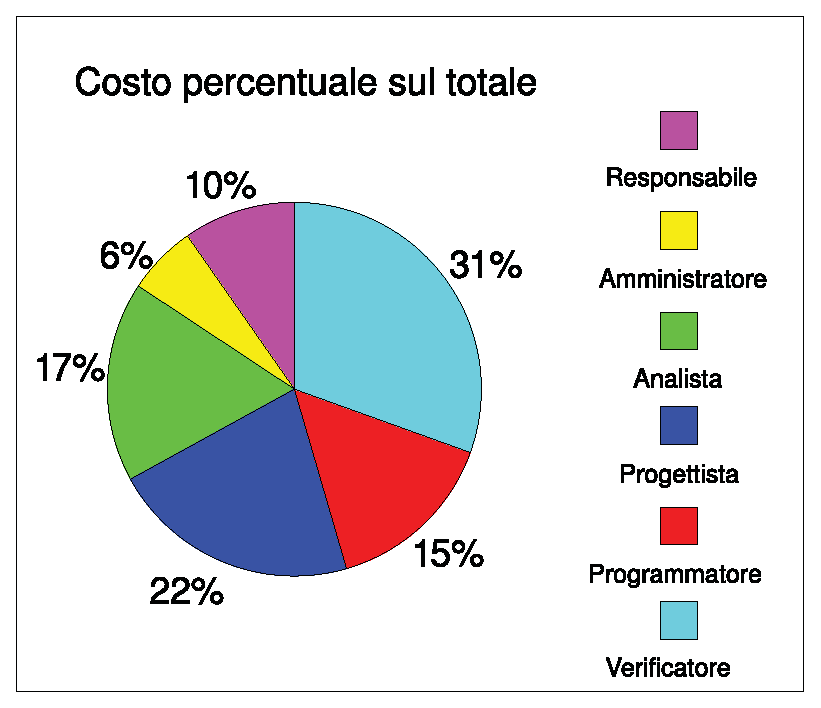
\includegraphics [width=1\textwidth] {costiPercentuali.eps}
\end{center}


\chapter{Diagramma di Gantt}
Alleghiamo due files denominati rispettivamente:
\begin {itemize} 
\item DiagrammaGantt\_0\_1.png che rappresenta l'impiego delle risorse nel tempo 
visualizzate giorno per giorno
\item DiagrammaGanttSettimanale\_0\_1.png che invece mostra l'impiego delle risorse
pi\'u globalmente organizzato per settimane
\end{itemize}

\begin{center}
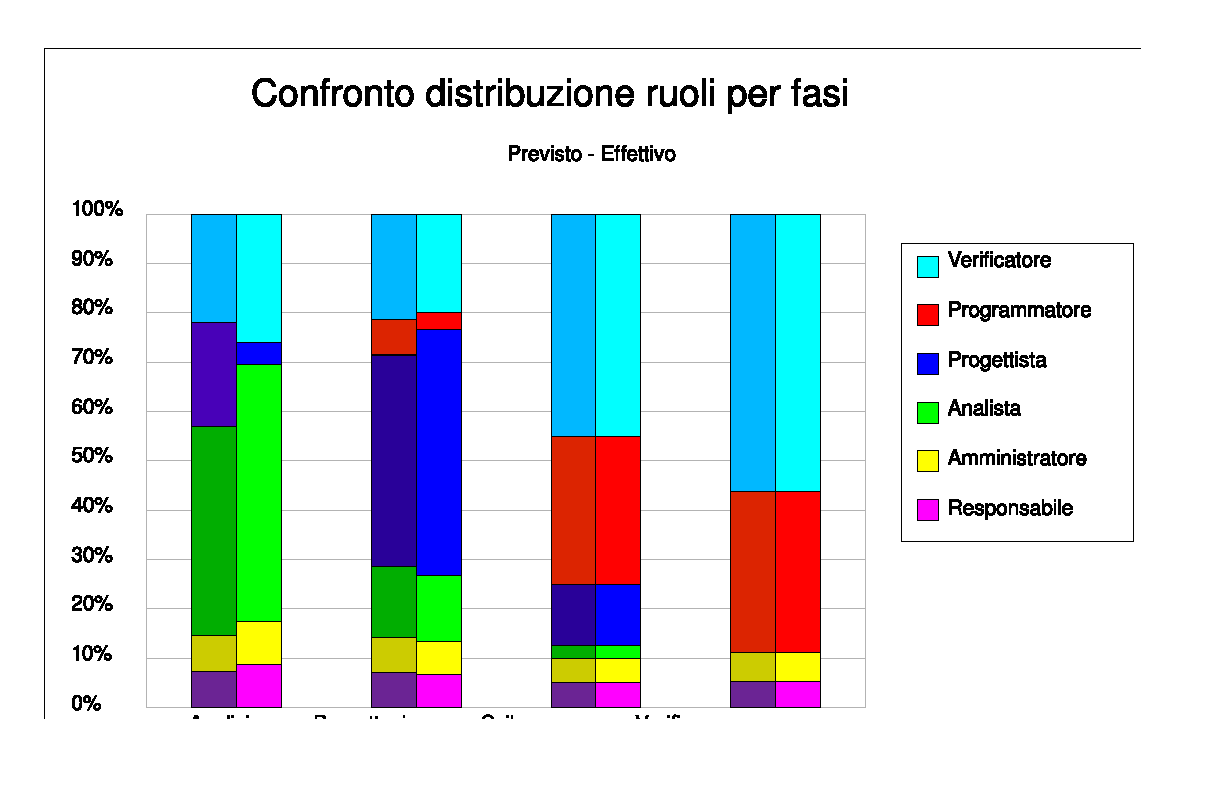
\includegraphics [width=1\textwidth] {confronto.eps}
\end{center}

\end{document}
	
